\subsection{AI Explainability as a purpose to traceability}
\label{sec:explainability}

In machine learning, the problem of reproducibility is manifold. Already because, for lack of international methodological standards, no one can verify the method by which your learning database was collected or the way in which the items were labelled. 
A critical question, because it is this dataset that provides the research context - or "environment" - for your algorithm: Without reliable data, an algorithm is worthless. And without an explainable algorithm, reliable data remains unsafe~\cite{beam2020-ai-reproduciblity-in-health,avital2018-realistic-evaluation-of-ai}. 
Lead AI scientists acknowledge that AI research today suffers a frenetic pace where scientific challenges becomes competitive arguments. There is a lack of rigorous standards for empirical work as well in results dissemination and the quest for knowledge has become a run for precision and recall derivatives. Under this process, researchers do not understand why one attempt at solving a problem worked and another failed. People implement and share techniques they do not remotely understand~\cite{sculley2018-winners-curse-progress-empirical-rigor}. Initiatives prone to qualify AI processes and results, such as the ReQuest tournament, focus on efficiency and software-hardware optimization rather than explainability. Traceability is not mentioned~\cite{request2018}. Approaches to machine learning epistemic uncertainty do not mention it either~\cite{hllermeier2019-aleatoric-and-epistemic-uncertiainty-in-ml}.\\

We wondered if AI-enabled software engineering suffers from the same issues. That is, we wanted to analyse whether recent advanced on the application of AI to improve the many software engineering tasks were also oblivious to explain and trace AI-enabled architecture decisions despite a global agreement in the AI community about the importance of explainability aspects.

To make a first step toward an answer to this question, we have run a second survey. This survey focuses on papers published in a representative set conferences proposing new AI techniques for software engineering to analyse whether they include explainability and/or traceability concerns as part of their proposal.

%As we said in the introduction, the use of AI in software development has brought some new challenges. As a final corollary to this work, we would like to see if the prominent qualities of traceability are prone to make AI-enabled systems more explainable. Are traceability approaches explicitly mentioned in work on AI-enabled software development? How can traceability assist AI-enabled systems become clearer? We answer this question with a short survey where we evaluate the quantity of literature covering this issue. 

\subsubsection{Survey method}
Following the same guidelines as for the previous survey, we followed the methodology presented by Kitchenham and Charters, with the purpose to filter papers from representative software engineering international venues (namely, the International Conference on Software Engineering (ICSE), the International Conference on Automated Software Engineering (ASE), and the Symposium on the Foundations of Software Engineering (FSE)) that mention explicitly the AI nature of their work. The query we applied on the DBLP database describes terms variations between machine learning, artificial intelligence, evolutionary computation. We also included variations of the terms "intelligent" and "smart". This process output 195 papers out of 109 proceedings. 

Here is the exact query we applied:
\begin{verbatim}
	^.*(([Dd]eep)|([Aa]rtificial[- ][Ii]ntelligence)|
	([Nn]eural [Nn]etwork)|([Mm]achine [Ll]earning)|
	[Ee]volutionary|AI|DL|[Ss]mart|[Ii]ntelligent).*
\end{verbatim}

We then applied the following inclusion and exclusion criteria to reach a selection of 81 papers relevant to our study.
\textit{Inclusion criteria}
\begin{enumerate}
	\item the work is a software engineering approach
	\item the work is from one of the three major software engineering venues (ICSE, FSE, or ASE)
	\item the work mentions artificial intelligence techniques
\end{enumerate}

\textit{Exclusion criteria}
\begin{enumerate}
	\item the paper is not about artificial intelligence techniques
	\item the paper is not a white paper
\end{enumerate}

%Literally:
%\begin{verbatim}^.*(([Dd]eep)|([Aa]rtificial[- ][Ii]ntelligence)|([Nn]eural [Nn]etwork)|
%([Mm]achine [Ll]earning)|
%[Ee]volutionary|AI|DL|[Ss]mart|[Ii]ntelligent).*\end{verbatim}

\begin{figure}[h]
		\centering
		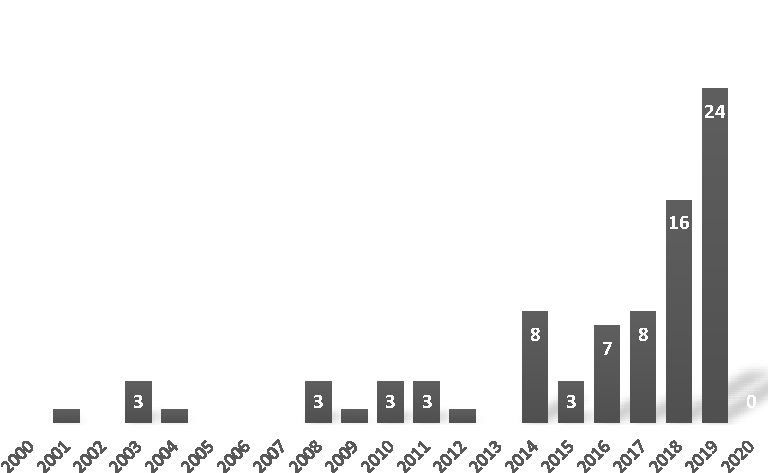
\includegraphics[width=.6\linewidth]{images/publicationyears-aiinse}
		\caption{Papers mentioning artificial intelligence in SE major venues. }
		\label{fig:publicationyears-ai}
\end{figure}

\subsubsection{Survey analysis}
We can see in \Fig{fig:publicationyears-ai} an exponential rise of the number of papers in the last years when. This contrasts with the gradual decrease of publications focused on traceability in the same period of time we have seen before (see \Fig{fig:publicationyears-tm}).

But, the key question is where these 81 papers do recognize the importance traceability or related concepts as part of their proposal. This is not the case, out of the 81 AI related papers collected in the main venues for software engineering research, only two use some kind of traceability to address functional quality of AI-enabled system. Clearly, traceability, recognized as a strong weapon for verification and accountability enhancement, has not got much attention in new AI-enabled techniques for software engineering. 
%One combines program execution and symbolic analysis to explore the execution paths of software programusing Deep Neural Networks (DNNs). In this paper, authors formalise coverage criteria for DNNs and then develop a coherent method for performing concolic testing to increase test coverage~\cite{Sun_2018-concolic-for-RNN}. In the second paper, symbolic execution is adapted into optimization problems representing the (non-)feasibility of paths. A machine learning algorithm then solves the problems. Authors show the method helps in black-box functions calls, between others, and thus is suitable for AI-enabled systems~\cite{Li_2016-symbolic-execution-feasibility}.

%\ugh{Yet AI explainability crisis would benefit from better traceability.}

%\textbf{Conclusion.} 
%AI is used for many things, including traceability. But in the software engineering realm, traceability is anything but used to aid and augment AI explainability.
%The inherent ability of artefacts to link which each others and to visualize these links explicitly is directly related to the time passed in validation and verification (inspection). We envision that explainability and accountability would gain at putting traceability as a core quality - of software development in general, and AI-enabled software in particular, and we call for more work in this area.

